% LaTeX template for the final master thesis

\documentclass[a4paper, 12pt]{book}
\pagestyle{plain}
\usepackage[a4paper, left=2.5cm, right=2.5cm, top=3cm, bottom=3cm]{geometry}
\usepackage{times}
\usepackage[latin1]{inputenc}
\usepackage[english]{babel}
\usepackage{url}
\usepackage{graphicx}
\usepackage{float}  									 % H for Figures positioning
\usepackage[nottoc, notlot, notlof, notindex]{tocbibind} % Index options
\usepackage{latexsym}  									 % LaTeX Logo
\usepackage{caption}
\usepackage{titlesec}
\usepackage{booktabs}
\usepackage{array}
\usepackage{enumitem}

\graphicspath{{./img/}}

\title{Implementation of a high availability solution based on Free Libre Open Source Software tools for Netnovation's Email and Collaboration System}
\author{Daniel H. G\'{a}mez V.}

\renewcommand{\baselinestretch}{1}  					% Interlining

\begin{document}

%=====================================
% COVER
%
\begin{titlepage}
  \begin{center}
  \begin{tabular}[c]{c c}
    
\includegraphics[scale=0.25]{logo_vect.eps}
    \begin{tabular}[b]{l}
      \Huge
      \textsf{UNIVERSIDAD} \\
      \Huge
      \textsf{REY JUAN CARLOS} \\
    \end{tabular}
  \end{tabular}
  \vspace{3cm}
  
  \Large
  Master in Free Libre Open Source Software\\
  \vspace{0.2cm}
  \large
  Academic Course 2014/2015 \\
  \vspace{0.4cm}
  Master Thesis \\
  \vspace{1cm}
  \LARGE
  Implementation of a high availability solution based on Free Libre Open Source Software tools for Netnovation's Email and Collaboration System \\
  \vspace{2cm}
  \large
  Author: DANIEL H. G\'{A}MEZ V.\\
  Tutor: DR. GREGORIO ROBLES
  
  \end{center}
\end{titlepage}

%=====================================
% LICENSE
%
{\raggedleft
(c) 2014, Daniel H. G\'{a}mez V.\\
 daniel.gamez@gmail.com\\
 This work is licensed under a\\
 Creative Commons Attributions 3.0 License
  \begin{figure}[H]
    {\raggedleft
    
\includegraphics[scale=0.80]{by-sa.png}\\
    \hfill http://creativecommons.org/licenses/by-sa/3.0/legalcode
    }
  \label{fig:logo}
  \end{figure}
}

%=====================================
% ABSTRACT
%
% \begin{abstract} This is the Abstract... \end{abstract}
% \chapter*{\centering Abstract}
\chapter*{Abstract}
\label{chap:abstract}
\addcontentsline{toc}{chapter}{Abstract}

This is the Abstract...

\noindent
Key words: Cluster, Corosync, DRBD, FLOSS, High Availability, Pacemaker, Zimbra

%=====================================
% ACKNOWLEDGEMENTS
%
\chapter*{Acknowledgements}
\label{chap:acknowledgements}
\addcontentsline{toc}{chapter}{Acknowledgements}

These are the Acknowledgements..

%=====================================
% CONTENTS
%
\tableofcontents  	% General Index
\listoffigures  	% Figures Index
\listoftables 		% Tables Index

%=====================================
% INTRODUCTION
%
\chapter{Introduction}
\label{chap:introduction}

Since year 2004 Netnovation\texttrademark \ is a Venezuelan SME, formed by a team of professionals in the areas of IT and telecommunications who adopted a business model based on consulting around FLOSS~\cite{Daffara2}, providing system integration, timely development and Software as a Service (SaaS) cloud services.

\begin{itemize}
	\item Disposition/document structure, the way the dissertation is going to be organized...
\end{itemize}



%=====================================
% PROBLEM STATEMENT 
%
\chapter{Problem statement}
\label{chap:problem}

Business continuity in the field of information technology is supported in a large extent by the uninterrupted operation of the systems used in productivity tasks~\cite{ISO}. These systems must be fault tolerant, so that operations have the least possible impact in the event that an unexpected incident occurs.\\

\noindent Nowadays there are increasingly more people and organizations using centralized remote systems that allow online access to resources and everyday services, this scheme is called cloud computing~\cite{Mell & Grance}. Through this type of services, end users whether individuals or corporations, are abstracted to support the infrastructure that this entails, giving responsibility to intermediary companies providing cloud services. So these intermediaries are the ones who must ensure the proper availability of the services, as well as factors such as communications security and redundancy of stored data, among many others.\\

\noindent In particular Netnovation is a SME in the field of information technologies, which provides private cloud services from data storage to hosting virtual private servers (VPS), including e-mail and collaboration servers. The latter is precisely one of the mainstays for the operations of the company, which employs mainly FLOSS to its internal systems, specifically using the FLOSS e-mail and collaboration suite Zimbra\texttrademark \footnote{\ http://www.zimbra.com}. One of the main problems that Netnovation faces is to ensure the communication and workflow continuity that is carried through this collaboration tool, as well as meet the SLAs offered to its customers over this software.\\

\noindent There are various software solutions offering high availability of services such as those provided by Zimbra, each one with its legal implications, associated costs and implementation difficulty \footnote{\ Some of these solutions will be addressed in Chapter~\ref{chap:related}}. A valid alternative is the integration of multiple tools in the field of FLOSS providing a framework to ensure  continuity of systems operation or business continuity. By doing it this way it is possible to adapt the different requirements and use different technologies to provide the most consistent solution to what is desired.\\

\noindent On previous occasions, Netnovation has managed to successfully consolidate most of its operations infrastructure adapting FLOSS, making it a wonderful idea to keep this scheme working. To achieve this, it is necessary to evaluate the state of the art in the field of systems that provide high availability, with the aim of offering an effective solution, all of this in accordance to the guidelines that have been proposed by the company.



\section{Justification / Motivation}
\label{sec:justification}


The factors that motivates this work are on one hand, give proper credit to business models based on FLOSS as those used by technology companies nowadays~\cite{Daffara2}, and on the other hand, show that private enterprise can be benefited by FLOSS, through a set of toolsets and mechanisms who allow obtaining robust solutions in accordance to technology needs.

\section{Objetives}
\label{subsec:objetives}

The overall objectives are:

\begin{itemize}
	\item Frame the FLOSS business model used by Netnovation
	\item Show various current alternatives provided by FLOSS at the corporate level
	\item Adapt the proposed solution to the guidelines established by Netnovation
	\item Establish an initial point reference for implementing high availability private cloud services offered by Netnovation
\end{itemize}

\noindent The specific objectives are:

\begin{itemize}
	\item Implement a high availability solution based on FLOSS for the e-mail and collaboration system Zimbra used by Netnovation
	\item Describe the methodology used for the selection of the solution to be implemented
	\item Describe the process undertaken to implement the selected solution
	\item Perform tests in a controlled laboratory environment and validate the correct operation of the solution in order to promote it to a production environment
\end{itemize}



\section{Scope}
\label{sec:scope}

The solution to be implemented consists of FLOSS tools that allow its adaptation to the current infrastructure of Netnovation, they are not intended to replace the elements of the existing operations  platform.\\

\noindent The methodology used for the selection of FLOSS tools that make the proposed solution is not intended to provide an exhaustive process that considers all possibilities in the area, but a flexible way that allows classify them qualitatively, justifying their choice through concrete metrics.\\

\noindent Having successfully implemented a high availability solution on the e-mail and collaboration system used by Netnovation, this will serve as a reference for providing high availability to other enterprise systems, but these other configurations are not covered in this exercise.\\


%=====================================
% PRECEDENTS / RELEATED TECHNOLOGIES / STATE OF THE ART
%
\chapter{Releated technologies}
\label{chap:related}

High Availability solutions based in FLOSS:\\

\noindent Commercial cluster software:
\begin{itemize}
	\item SUSE Linux Enterprise High Availability Extension
	\item openSUSE High Availability
	\item Red Hat Enterprise Linux Cluster
\end{itemize}

\noindent Standalone FLOSS tools:
\begin{itemize}
	\item Linux-HA\footnote{\url{http://www.linux-ha.org/wiki/Main_Page}}
\end{itemize}


%=====================================
% METHODOLOGY
%
\chapter{Methodology}
\label{chap:methodology}

The followed roadmap to achieve the objectives outlined is a set of guidelines and suggestions for the adoption of FLOSS within SMEs~\cite{Daffara1}, in the sense that a methodology is not an exact formula but a set of practices. At using this model, companies find a supporting guide from the initial selection and adoption of FLOSS within the IT infrastructure and even to the consolidation of business models around open source.\\

\noindent On the one hand, the guidelines proposed by Daffara suggest a research method by collecting and read as much information related to the project is available and select the appropriate solution from a matching set that fulfill the requirements. On the other hand this dissertation also contemplates an open and standard framework to select the technologies to be used, this is the light weight model OpenBRR~\cite{Wasserman et. all}, which performs a quick and flexible assessment over software tools considered.\\

\noindent Additionally, and following a practical formal approach, applying a model of technology acceptance such as the Lazy User Model (LUM)~\cite{Collan and Tetard} is possible to frame the process by which are chosen the technological tools that will make up the solution that meets user requirements, which in this case is being represented by the company Netnovation. This model focuses on user needs and the demanded effort when selecting a solution to a problem from a set of possible solutions.\\

LUM: ``According to the lazy user model, a user is likely to choose the solution that requires the least effort
The selection between one solution and another is known as 'Switching Cost', which tell us that the user examines this cost in terms of time, energy and money when considering how to use a new solution. The LUM proposes that technology acceptance is impacted by the principle of least effort."

\section{OpenBRR}
\label{sec:openbrr}


%=====================================
% ARCHITECHTURE
%
\chapter{Architecture}
\label{chap:architecture}

In order to provide IT services to customers, considering software services hosted in an on-line remote location, Netnovation requires a proper software and hardware infrastructure to operate. Some of these services are from VPS, Data Storage Systems, Customer Relationship Management Systems (CRM), Email and Collaboration Systems, to Voice over IP PBX systems. Both parties, software infrastructure and product services offered are based on FLOSS.\\

\noindent In particular the Zimbra server to which a high availability schema is been configured, resides into this architecture, and it is consistent with the company's principles and business model, which is why it is useful to understand the environment to which it belongs.


\section{Company Infrastructure}
\label{sec:infrastructure}

Currently the services are offered from two DataCenters (DC1 and DC2) geographically distributed with the aim of guarantee data redundancy. Assuming that communication with the main DC is lost, it has been defined a procedure that allows the restoration of services in the other DC, with the disadvantage that it is a manual procedure that requires administrators intervention.

\section{Existent Hardware}
\label{sec:hardware}

Each DC has an average of seven Dell\texttrademark \ PowerEdge Racked Servers with different capacities, interconnected via communication devices that provide various services analogously.\\

There is a Dell PowerEdge 2850/2950 server serving as firewall and main router on each DC. On the one hand it has a WAN 1000Mbps interface, which is connected through UTP Cat-6 wired to 24 PoE ports Switches Netgear FS728TPv1 Gigabit. Physical servers are installed in 20U rack cabinets. These servers range from models Dell PowerEdge 1950, R510 to R710, have Intel Xeon CPUs within 24 and 64 cores, count with 8 to 64GB of RAM, and also have SCSI HDD with capacities between 100GB and 2,5TB.

\section{Company Network Scheme}
\label{sec:network}

The housing services leased by the providers offer a pool of public IPv4 addresses that are handled by the main router on each DC facility. DC1 and DC2 are interconnected by a VPN through WAN, each of them associated to a different private Class B network internally. To the LAN Ethernet ports of the switches are connected the physical servers of the private network with transfer speed rates of 100/1000Mbps. The overall interconnection scheme can be appreciated in Figure~\ref{fig:network}.

\begin{figure}[H]
  \centering
  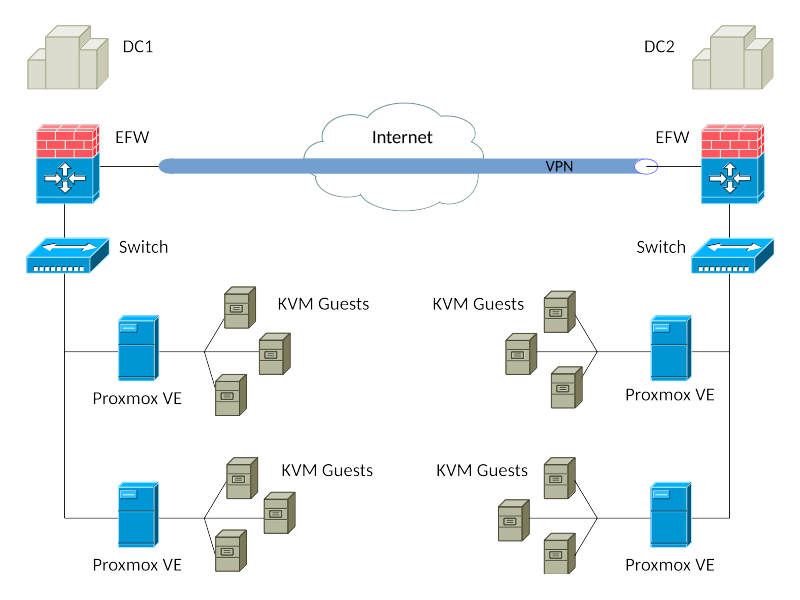
\includegraphics[scale=0.50]{network_scheme.png}
  \caption[Network interconnection scheme]{Network interconnection scheme}
  \label{fig:network}
\end{figure}

\section{Software Supporting the Infrastructure}
\label{sec:software}

In Table~\ref{table:technologies} there are some software solutions currently used by Netnovation that are related with the required architecture to provide IT cloud-oriented services, with a brief description and legal licensing information for each one of them.

\begin{table}
  \centering
  \begin{tabular}{ | r m{10cm} | }
  
    \hline    
    \multicolumn{2}{|c|}{\textbf{UTM Endian Firewall}}\\
    \hline
    Company: & Endian S.r.l. \\
    Industry: & Unified Threat Management \\
    License: & GNU GPL \\
    Website: & endian.com \\
    Description: & A linux security distribution with full featured Unified Threat Management functionality. Include a stateful packet inspection firewall, application-level proxies for various protocols, antivirus support, virus and spam-filtering for email traffic, content filtering of Web traffic, also an OpenVPN solution. Distribution based on Red Hat. \\
    Supported Platforms: & GNU/Linux \\
    Commercial support: & annual subscription \\
    
    \hline    
    \multicolumn{2}{|c|}{\textbf{Proxmox VE}}\\
    \hline
    Company: & Proxmox Server Solutions GmbH \\
    Industry: & Server Virtualization \\
    License: & GNU Affero and GPLv3 \\
    Website: & pve.proxmox.com \\
    Description: & Virtualization management solution for servers, based on KVM and containers Server Virtualization Platform, provides KVM and OpenVZ hypervisors. Distribution based on Debian. \\
    Supported Platforms: & GNU/Linux \\
    Commercial support: & annual subscription \\
    
    \hline    
    \multicolumn{2}{|c|}{\textbf{FreeNAS}}\\
    \hline
    Company: & iXsystems, Inc. \\
    Industry: & Computer Storage \\
    License: & BSD 2-Clause \\
    Website: & freenas.org \\
    Description: & Network-attached storage server, supporting many network and storage protocols such as Samba and NFS. Also supports ZFS. Distribution based on FreeBSD. \\
    Supported Platforms: & BSD Unix \\
    Commercial support: & custom quotes and support tickets \\
    \hline
    \multicolumn{2}{|c|}{\textbf{Zabbix}}\\
    \hline
    Company: & Zabbix SIA \\
    Industry: & IT Monitoring \\
    License: & GNU GPLv2 \\
    Website: & zabbix.com \\
    Description: & Solution for monitoring of networks, applications and databases. \\
    Supported Platforms: & GNU/Linux \\
    Commercial support: & custom quotes and support tickets \\
    \hline
  \end{tabular}
\caption{Software Supporting the Infrastructure}
\label{table:technologies}
\end{table}



%=====================================
% IMPLEMENTED TECHNOLOGIES
%
\chapter{Implemented technologies}
\label{chap:implemented}

The following software tools represent the key elements on which it has been possible to implement a comprehensive high availability solution. 

\begin{itemize}
	\item Red Hat Enterprise Linux Server
\end{itemize}

\noindent GNU/Linux enterprise-oriented distribution providing a very stable base system, vast documentation and proper support from manufacturer, released as FLOSS mainly under the terms of the GNU Lesser General Public License 2.1, except for some optional components. In order to be specific in this exercise, the Linux kernel 2.6.32-431.el6.x86\_64 that is included by the RHEL version 6.5 was used.

\begin{itemize}
	\item Zimbra Collaboration System (ZCS)
\end{itemize}

\noindent Server and client collaboration software, supporting e-mail, contacts, calendar, documents, push synchronization, and many other enterprise features related to groupware. The software is FLOSS released under the terms of the Common Public Attribution License version 1 and the GNU General Public License version 2 (GPLv2). The exact version implemented was ZCS FOSS  8.0.7\_GA\_6021.RHEL6\_64.

\begin{itemize}
	\item Distributed Replicated Block Device (DRBD)
\end{itemize}

\noindent A distributed replicated storage system for Linux, implemented as several userspace management applications and shell scripts, used to provide data redundancy. DRBD software is FLOSS released under the terms of the GNU GPLv2. 

\begin{itemize}
	\item Corosync
\end{itemize}

\noindent It is released as FLOSS under the 3-clause BSD License. This software provides features based on C programming language implementing high availability within applications, through virtual synchrony for replicated state machines, simple availability handling responsible for applications restart when fail, it keeps configuration and statistics in a memory database providing the ability to set, retrieve, and receive change notifications of information, and a quorum system that notifies applications when it is achieved or lost.

\begin{itemize}
	\item Pacemaker
\end{itemize}

\noindent A FLOSS high availability resource manager software released under GNU GPLv2. This software was part of the Linux-HA project until 2007, then was split out to be its own project. It implements APIs for resources control, including the Open Cluster Framework (OCF). It is used on computer clusters since 2004.

\begin{itemize}
	\item Cluster Resource Manager Shell (CRMsh\footnote{http://crmsh.github.io}) and Pacemaker Configuration System (PCS\footnote{https://github.com/feist/pcs})
\end{itemize}

\noindent Initially, the CRMsh was distributed as part of the Pacemaker project, but it was split into its own separate project in 2011. Also as CRMsh, PCS is a command-line interface to the Pacemaker cluster resource management stack.

\begin{itemize}
	\item Cluster Configuration System (CCS)
\end{itemize}

\noindent Manages the cluster configuration and provides information to other cluster components. Runs in each cluster node and makes sure that the cluster configuration file in each cluster node is up to date. In Figure~\ref{fig:ccs} (\small {took from \url{https://access.redhat.com/documentation/en-US/Red_Hat_Enterprise_Linux/4/html/Cluster_Suite_Overview/images/}}) is represented a CCS overview.

\begin{figure}[H]
  \centering
  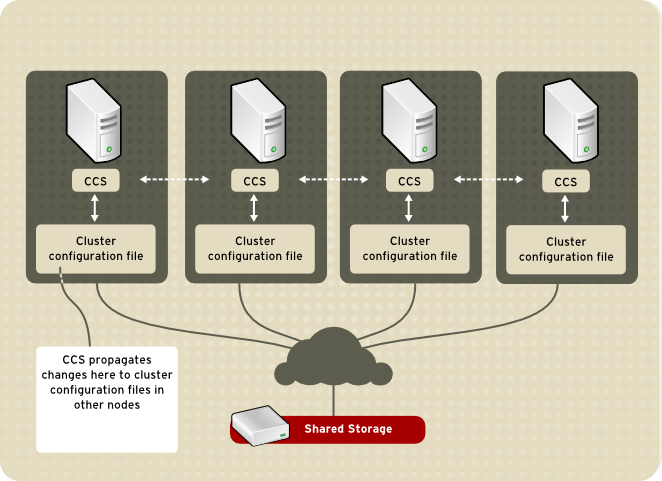
\includegraphics[scale=0.50]{ccs-overview.png}
  \caption[CCS overview]{CCS overview}
  \label{fig:ccs}
\end{figure}

\begin{itemize}
	\item Cluster Manager (CMAN\footnote{https://www.sourceware.org/cluster/cman/})
\end{itemize}

\noindent A set of kernel patches and a userspace program, formed by a Connection Manager (cnxman) and a Service Manager (sm). The first one handles membership, messaging, quorum, event notification and transitions, and the second one is responsible for instances of external systems. It combines some functionalities provided by CRMsh, PCS and CCS.


%=====================================
% IMPLEMENTATION
%
\chapter{Implementation}
\label{chap:implementation}

This section is intended to provide technical documentation in the process of implementing high availability in a FLOSS Zimbra Collaboration System (ZCS). The scope of this implementation is limited to the following software components and versions:
\begin{itemize}
	\setlength{\itemsep}{0pt}
	\item Red Hat Enterprise Linux Server release 6.5 (Santiago)
	\item GNU/Linux 2.6.32-431.el6.x86\_64
	\item zcs 8.0.7\_GA\_6021.RHEL6\_64 FOSS edition
	\item drbd 8.4.3-33
	\item corosync 1.4.5-2.2
	\item pacemaker 1.1.10-14
	\item pcs 0.9.90-2
	\item crmsh 1.2.5-0
	\item ccs 0.16.2-69
	\item cman 3.0.12.1-59
\end{itemize}

\noindent The defined cluster consists of two nodes which will be referenced as Astapor and Braavos in the domain got.com (as in the novel Game of Thrones). These nodes are virtual machines hosted on two Proxmox Virtual Environment servers based on KVM virtualization, which are installed on separate physical machines in the same LAN to avoid single point of failure. The proposed scheme is conceptually similar to the observed in Figure~\ref{fig:ha-cluster}.

\begin{figure}[H]
  \centering
  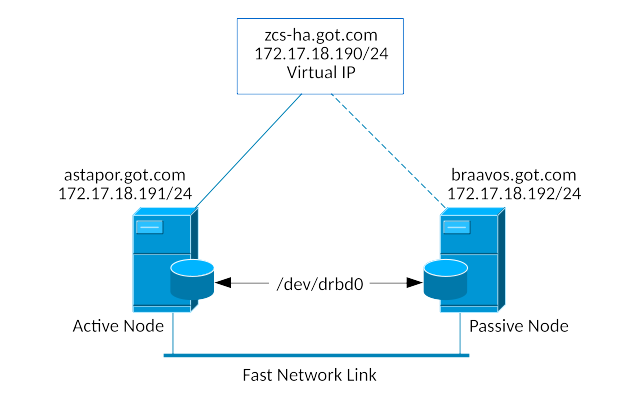
\includegraphics[scale=0.50]{two_nodes_ha_cluster.png}
  \caption[Two nodes HA cluster]{Two nodes HA cluster}
  \label{fig:ha-cluster}
\end{figure}





%=====================================
% RESULTS AND DISCUSSION
%
\chapter{Results and discussion}
\label{chap:results}

Text..


%=====================================
% CONCLUSIONS
%
\chapter{Conclusions and future work}
\label{chap:conclusions}

Text..

%=====================================
% REFERENCES
%
\renewcommand{\bibname}{References}

\begin{thebibliography}{25}
  \bibliographystyle{alpha}

  \bibitem{Fogel} Fogel, Karl. \textit{Producing Open Source Software: How to Run a Successful Free Software Project}. O'Reilly, 2005.

  \bibitem{Raymond} Raymond, Eric. \textit{The Cathedral and the Bazaar}. O'Reilly, 1999.

\end{thebibliography}

%=====================================
% APPENDIX
%
\appendix
\chapter{Title of appendix 1}
\label{app:apendix1}


\end{document}